\documentclass{beamer}
\usepackage{xcolor}
% \usetheme{Marburg}
\usecolortheme{orchid}
\usepackage{pifont}
\usepackage{changepage}
\usepackage[
backend=biber,
style=alphabetic,
]{biblatex}
\addbibresource{main.bib}
\usepackage{hyperref, xcolor, cmbright,diagbox,colortbl,tikz,graphicx,algorithm2e,cancel,verbatim, graphicx,
listings,float,amsmath,amssymb,array,subfiles,bussproofs,
rotating,MnSymbol,hyperref,mathtools,subcaption,caption}
\usetikzlibrary{overlay-beamer-styles}
\usetikzlibrary{automata, positioning,graphs,shapes, arrows, calc}

\newcommand{\set}[1]{\{#1\}}
\newcommand{\vertex}[2]{%
  \begin{tikzpicture}[baseline=-1ex]%
    \node [rectangle,rounded corners=2mm,inner sep=0.5mm,fill=#2] {$#1$};%
  \end{tikzpicture}%
}
\newcommand{\graphbox}[8]{
  \begin{scope}[xshift=#2,yshift=#3]
    \draw [rounded corners=2mm] (0,0) rectangle (#4,-#5);
    \node at (0,0mm) [anchor=north west,inner sep=1mm] {#1};
    \begin{scope}[xshift=#4/2+#6,yshift=#7] 
    #8
    \end{scope}
  \end{scope}
}

\newcommand{\nodeGraph}{
	\,\begin{tikzpicture}[baseline=-.6ex]
		\node (x) [circle,inner sep=0,outer sep=1mm,minimum size=0.7mm,fill=black] {};
	\end{tikzpicture}\, 
}

 
\newcommand{\edgeGraph}[1]{
	\,\begin{tikzpicture}[baseline=-.6ex]
		\node (x) [circle,inner sep=0,outer sep=1mm,minimum size=0.7mm,fill=black] {};
		\node (y) [circle,inner sep=0,outer sep=1mm,minimum size=0.7mm,fill=black, right of=x, xshift=-3mm] {};
		\draw [-] (x) -- node[midway,above] {$#1$} (y) ;
	\end{tikzpicture}\,
}

%%% end endrullis 


\graphicspath{ {.} }

\title{Termination of Injective DPO Graph Rewriting Systems using Subgraph Counting}
\setbeamertemplate{footline}[frame number]
\begin{document}
\date{\today}

\institute[VFU] % (optional)
{
    Qi QIU \\
	Supervisor: Xavier URBAIN\\
	Universite Claude Bernard Lyon 1, CNRS, INSA Lyon,\\ LIRIS, UMR5205, 69622 Villeurbanne, France \\
    Univ. Grenoble Alpes, CNRS, Grenoble INP,\\
               LIG, 38000 Grenoble, France\\
	% Projet SAPPORO
}  

\maketitle

\section{Master's Thesis Projects}
\subsection{Impact of Clause Sharing Strategies in Parallel SAT Solvers}
\begin{frame}
        \tableofcontents[currentsubsection]
\end{frame}
\begin{frame}
    \begin{adjustwidth}{-1.5cm}{0cm}
    \begin{description}
        \item[] SAT solver: miniSAT
        \item[] Parallelization
        \item[] Single Program Multi Data (SPMD)
        \item[] Message Passing Interface (MPI) / C++
        \item[] A processor / a miniSAT instance / a strategy
        \item[] Impact of Clause Sharing Strategies
                 \begin{itemize} 
                    \item limit the size of the clauses to be shared
                    \item share with different number of neighbours
                    \item ...
                \end{itemize}
    \end{description}
\end{adjustwidth}
\end{frame}


\subsection{Formal Verification of Theorem Proving Methods}
\begin{frame}
    \tableofcontents[currentsubsection]
\end{frame}

\begin{frame}{Automated Theorem Proving by Saturation}
    \begin{adjustwidth}{-1.5cm}{0cm}
        \begin{description}
            \item Proving $\vdash F$ by proving $\lnot F \vdash \bot$
            \item Example:
                \begin{itemize}
                    \item for proving $\vdash p \lor \lnot p$
                    \item calculate $\lnot(p \lor \lnot p) = \lnot p \land p$
                    \item we have $\{\lnot p, p\} \vdash \bot$
                    \item thus $\vdash p \lor \lnot p$
                \end{itemize}
        \end{description}
    \end{adjustwidth}
\end{frame}

\begin{frame}{Given Clause Procedure}
    An automated theorem prover by saturation needs to 
    \begin{itemize}
        \item maintain a set of clauses $S$ 
        \item deduce new clauses from $S$
        \item delete redundant clauses from $S$
    \end{itemize}

    Given Clause Procedure (GC) is a set of rules for deciding
    \begin{itemize}
        \item which clauses to keep in $S$
        \item which clauses to use for deducing new clauses
    \end{itemize}
    % \begin{adjustwidth}{-1.5cm}{0cm}
    %      \begin{description}
    %         \item[] Maintain a set of clauses $S'$ and a set of given clauses $G$
    %         \item[] $S'$ is initialy $\empty$ 
    %         \item[] $G$ is initialy $S$
    %         \item[] at each iteration
    %             \begin{itemize}
    %                 \item take a clause, called \textcolor{red}{given clause}, $c \in G$
    %                 \item add resolvents of $c$ with clauses in $S'$ to $G$
    %                 \item deduce new clauses using $c$ and clauses in $S'$ and add them to $G$
    %                 \item move $c$ to $S'$
    %                 \item remove $c$ and redundant clauses from $G$
    %                 \item $\dots$
    %             \end{itemize} 
    %     \end{description}
    % \end{adjustwidth}
\end{frame}

\begin{frame}{Framework for Saturation Theorem Proving}
Given Clause Procedure (GC) 
\begin{itemize}
    \item Process:
        \begin{itemize}
            \item $\mathcal{N} \cup \mathcal{M} \implies_{\text{GC}} \mathcal{N} \cup \mathcal{M}'$ 
            where $\dots$
            % \(\mathcal{M} \subseteq \text{Red}_F^{\bigcap G_L, \square}(\mathcal{N} \cup \mathcal{M}')\) 
            % and \(\mathcal{M}'_{\text{active}} = \emptyset\) 
        \end{itemize}
    \item INFER:
        \begin{itemize}
            \item $\mathcal{N} \cup \{(C, l)\} \implies_{\text{GC}} \mathcal{N} \cup \{(C, \text{active})\} \cup \mathcal{M}$ where $\dots$  
        %     where \( l \neq \text{active}, \mathcal{M}_{\text{active}} = \emptyset \), 
        %     and $F_{\text{inf}}(\lfloor\mathcal{N}_{\text{active}}\rfloor, \{C\}) \subseteq \text{Red}_{\opn{I}}^{\bigcap G}(\lfloor\mathcal{N}\rfloor \cup \{C\} \cup \{\mathcal{M}\})
        % $
        \end{itemize}
\end{itemize}
 
 A Comprehensive Framework for Saturation Theorem Proving,  
Waldmann U., Tourret S., Robillard S., Blanchette J. (IJCAR 2020)
    \begin{itemize}
        \item Isabelle/HOL framework
        \item formalization of GC
        \item formalization of LGC
    \end{itemize}
\end{frame}

\begin{frame}{4 Variants employed by different Theorem Provers}

\begin{enumerate}
    \item Otter-loop(OL) : a refinement of GC
    \item iProver-loop(IL) : an extension of OL
    \item Discount-loop(DL) : a refinement of LGC
    \item Zipperposition-loop(ZL) : an extension of DL
\end{enumerate}
Correctness: Can any formula provable by a variant also be proved by GC?

\end{frame}

\begin{frame}{Contribution}
    \begin{adjustwidth}{-2cm}{0cm} 
        \begin{description}
            \item[] \textcolor{red}{Formalization} of the variants in Isabelle/HOL
            \item[] Proving their \textcolor{red}{correctness} in Isabelle/HOL
            \item[] International Conference on Automated Deduction 2023 (CADE-29)
        \end{description}
    \end{adjustwidth}
\end{frame}


\section{Doctoral Research: Termination of Graph Relabeling Systems}

\subsection{DPO Graph Rewriting and Termination}
\begin{frame}
   \tableofcontents[currentsubsection]
\end{frame}
\begin{frame}{DPO Graph Rewriting and Termination}
  \begin{description}
    \item[Edge-labeled directed graphs]
    \item[DPO graph rewriting rule]
  \end{description}
  \begin{center} 
                \resizebox{0.7\textwidth}{!}{
                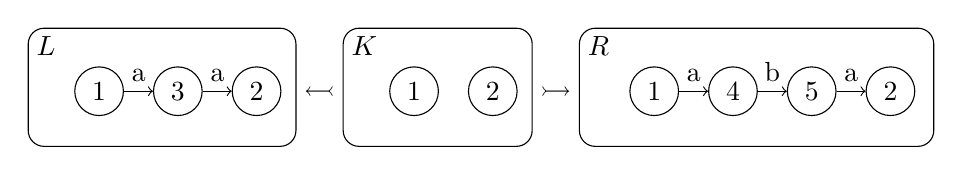
\begin{tikzpicture}
                    \graphbox{$L$}{0mm}{0mm}{34mm}{15mm}{2mm}{-5mm}{
                        \coordinate (o) at (0mm,-3mm); 
                        \node[draw,circle] (l1) at ($(o)+(-10mm,0mm)$) {1};
                        \node[draw,circle] (l2) at ($(l1)+(2,0)$) {2};
                        \node[draw,circle] (l3) at ($(l1) + (1,0)$) {3};
                        \draw[->] (l1) -- (l3) node[midway,above] {a};
                        \draw[->] (l3) -- (l2) node[midway,above] {a};
                    }     
                    \graphbox{$K$}{40mm}{0mm}{24mm}{15mm}{2mm}{-5mm}{
                        \coordinate (o) at (5mm,-3mm); 
                        \node[draw,circle] (l1) at ($(o)+(-10mm,0mm)$) {1};
                        \node[draw,circle] (l2) at ($(l1)+(1,0)$) {2};
                        % \node[draw,circle] (l3) at ($(l1) + (1,0)$) {$\ $};
                        % \draw[->] (l1) -- (l3) node[midway,above] {a};
                        % \draw[->] (l3) -- (l2) node[midway,above] {a};
                    }    
                    \graphbox{$R$}{70mm}{0mm}{45mm}{15mm}{2mm}{-5mm}{
                        \coordinate (o) at (-5mm,-3mm); 
                        \node[draw,circle] (l1) at ($(o)+(-10mm,0mm)$) {1};
                        \node[draw,circle] (l2) at ($(l1)+(3,0)$) {2};
                        \node[draw,circle] (l3) at ($(l1) + (1,0)$) {4};
                        \node[draw,circle] (l4) at ($(l1) + (2,0)$) {5};
                        \draw[->] (l1) -- (l3) node[midway,above] {a};
                        \draw[->] (l3) -- (l4) node[midway,above] {b};
                        \draw[->] (l4) -- (l2) node[midway,above] {a};
                    }    
                    \node () at (37mm,-8mm) {$\leftarrowtail$};
                    \node () at (67mm,-8mm) {$\rightarrowtail$};
                    % \draw[>->] (51mm,2mm) -- (52mm,3mm);
                \end{tikzpicture}
                }
            \end{center}
  \begin{description}
    \item[Graph transformation using DPO rewriting rule]
  \end{description}
   \begin{center}
    \resizebox{0.7\textwidth}{!}{
      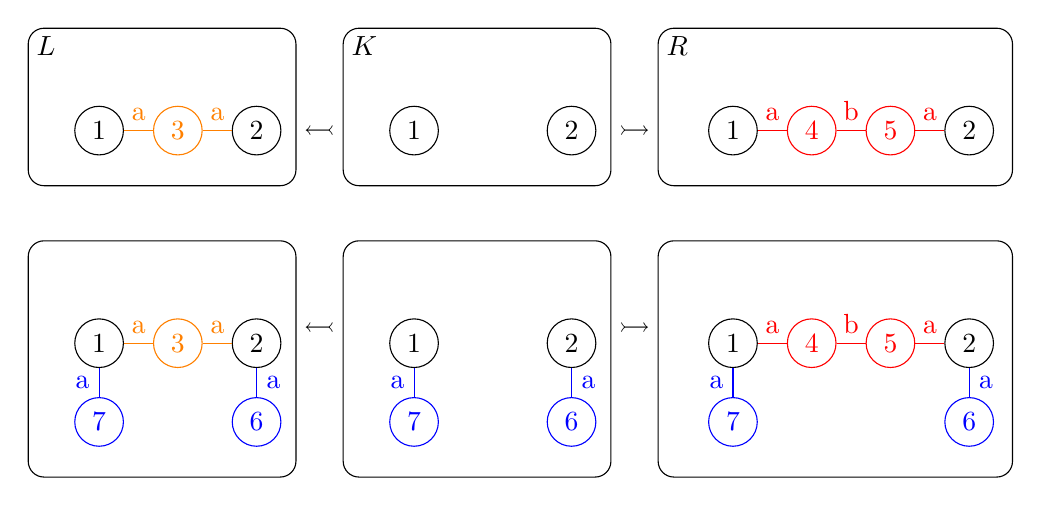
\begin{tikzpicture}
              \graphbox{\( L  \)}{0mm}{5mm}{34mm}{20mm}{2mm}{-5mm}{
                  \coordinate (o) at (0mm,-8mm); 
                  \node[draw,circle] (l1) at ($(o)+(-10mm,0mm)$) {1};
                  \node[draw,circle] (l2) at ($(l1)+(2,0)$) {2};
                  \node[orange,draw,circle] (l3) at ($(l1) + (1,0)$) {3};
                  \draw[orange] (l1) -- (l3) node[midway,above] {a};
                  \draw[orange] (l3) -- (l2) node[midway,above] {a};
              } 

              \graphbox{\( K \)}{40mm}{5mm}{34mm}{20mm}{2mm}{-5mm}{
                  \coordinate (o) at (0mm,-8mm); 
                  \node[draw,circle] (l1) at ($(o)+(-10mm,0mm)$) {1};
                  \node[draw,circle] (l2) at ($(l1)+(2,0)$) {2};
              }  

              \graphbox{\(  R \)}{80mm}{5mm}{45mm}{20mm}{2mm}{-5mm}{
                  \coordinate (o) at (-5mm,-8mm); 
                  \node[draw,circle] (l1) at ($(o)+(-10mm,0mm)$) {1};
                  \node[draw,circle] (l2) at ($(l1)+(3,0)$) {2};
                  \node[red,draw,circle] (l3) at ($(l1) + (1,0)$) {4};
                  \node[red,draw,circle] (l4) at ($(l1) + (2,0)$) {5};
                  \draw[red] (l1) -- (l3) node[midway,above] {a};
                  \draw[red] (l3) -- (l4) node[midway,above] {b};
                  \draw[red] (l4) -- (l2) node[midway,above] {a};
              }    

              \graphbox{\(   \)}{0mm}{-22mm}{34mm}{30mm}{2mm}{-10mm}{
                  \coordinate (o) at (0mm,-3mm); 
                  \node[draw,circle] (l1) at ($(o)+(-10mm,0mm)$) {1};
                  \node[draw,circle] (l2) at ($(l1)+(2,0)$) {2};
                  \node[draw,circle,orange] (l3) at ($(l1) + (1,0)$) {3};
                  \node[blue, draw,circle] (l4) at ($(l2) + (0,-1)$) {6};
                  \draw[orange] (l1) -- (l3) node[midway,above] {a};
                  \draw[orange] (l3) -- (l2) node[midway,above] {a};
                  \draw[blue] (l2) -- (l4) node[midway,right] {a};
                  \node[blue,draw,circle] (l6) at ($(l1) + (0,-1)$) {7};
                  \draw[blue] (l1) -- (l6) node[midway,left] {a};
              }    

              \graphbox{\(   \)}{40mm}{-22mm}{34mm}{30mm}{2mm}{-10mm}{
                  \coordinate (o) at (0mm,-3mm); 
                  \node[draw,circle] (l1) at ($(o)+(-10mm,0mm)$) {1};
                  \node[draw,circle] (l2) at ($(l1)+(2,0)$) {2};
                  \node[blue,draw,circle] (l4) at ($(l2) + (0,-1)$) {6};
                  \draw[blue] (l2) -- (l4) node[midway,right] {a};
                  \node[blue,draw,circle] (l6) at ($(l1) + (0,-1)$) {7};
                  \draw[blue] (l1) -- (l6) node[midway,left] {a};
              }    

              \graphbox{\(  \)}{80mm}{-22mm}{45mm}{30mm}{2mm}{-10mm}{
                  \coordinate (o) at (-5mm,-3mm); 
                  \node[draw,circle] (l1) at ($(o)+(-10mm,0mm)$) {1};
                  \node[draw,circle] (l2) at ($(l1)+(3,0)$) {2};
                  \node[draw,circle,red] (l3) at ($(l1) + (1,0)$) {4};
                  \node[draw,circle,red] (l4) at ($(l1) + (2,0)$) {5};
                  \node[blue,draw,circle] (l5) at ($(l2) + (0,-1)$) {6};
                  \node[blue,draw,circle] (l6) at ($(l1) + (0,-1)$) {7};
                  \draw[blue] (l1) -- (l6) node[midway,left] {a};
                  \draw[red] (l1) -- (l3) node[midway,above] {a};
                  \draw[red] (l3) -- (l4) node[midway,above] {b};
                  \draw[red] (l4) -- (l2) node[midway,above] {a};
                  \draw[blue] (l2) -- (l5) node[midway,right] {a};
              }    

              \node () at (37mm,-8mm) {\( \leftarrowtail \)}; % K -> L
              \node () at (77mm,-8mm) {\( \rightarrowtail \)}; % K -> R
              \node () at (17mm,-18mm) {\(  \downarrowtail \)};
              \node () at (37mm,-33mm) {\( \leftarrowtail \)};
              \node () at (52mm,-18mm) {\( \downarrowtail \)};
              \node () at (92mm,-18mm) {\( \downarrowtail \)};
              \node () at (77mm,-33mm) {\( \rightarrowtail \)}; % C -> H
      \end{tikzpicture}
      }
   \end{center}
  \begin{description}
    \item[Termination of DPO graph rewriting rule] 
  \end{description}
\end{frame}

\begin{frame}{DPO Graph Rewriting System: Example}

\begin{center} 
                \resizebox{0.7\textwidth}{!}{
                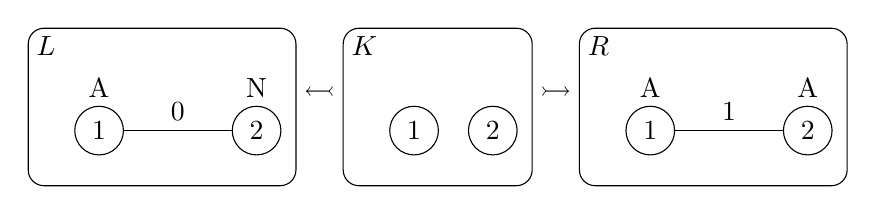
\begin{tikzpicture}
                    \graphbox{$L$}{0mm}{0mm}{34mm}{20mm}{2mm}{-5mm}{
                        \coordinate (o) at (0mm,-8mm); 
                        \node[draw,circle] (l1) at ($(o)+(-10mm,0mm)$) {1};
                        \node[draw,circle] (l2) at ($(l1)+(2,0)$) {2};
                        \draw ($(o)+(-10mm,3mm)$) node[above] {A};
                        \draw ($(l1)+(2,3mm)$) node[above] {N};
                        \draw[-] (l1) -- (l2) node[midway,above] {0};
                    }     
                    \graphbox{$K$}{40mm}{0mm}{24mm}{20mm}{2mm}{-5mm}{
                        \coordinate (o) at (5mm,-8mm); 
                        \node[draw,circle] (l1) at ($(o)+(-10mm,0mm)$) {1};
                        \node[draw,circle] (l2) at ($(l1)+(1,0)$) {2};
                        % \node[draw,circle] (l3) at ($(l1) + (1,0)$) {$\ $};
                        % \draw[->] (l1) -- (l3) node[midway,above] {a};
                        % \draw[->] (l3) -- (l2) node[midway,above] {a};
                    }    
                    \graphbox{$R$}{70mm}{0mm}{34mm}{20mm}{2mm}{-5mm}{
                            \coordinate (o) at (0mm,-8mm); 
                        \node[draw,circle] (l1) at ($(o)+(-10mm,0mm)$) {1};
                        \node[draw,circle] (l2) at ($(l1)+(2,0)$) {2};
                        \draw ($(o)+(-10mm,3mm)$) node[above] {A};
                        \draw ($(l1)+(2,3mm)$) node[above] {A};
                        \draw[-] (l1) -- (l2) node[midway,above] {1};
                    }    
                    \node () at (37mm,-8mm) {$\leftarrowtail$};
                    \node () at (67mm,-8mm) {$\rightarrowtail$};
                    % \draw[>->] (51mm,2mm) -- (52mm,3mm);
                \end{tikzpicture}
                }
            \end{center}
    Example: the construction of a spanning tree
        \begin{overlayarea}{\textwidth}{3cm}
            \centering
            \begin{onlyenv}<1>
                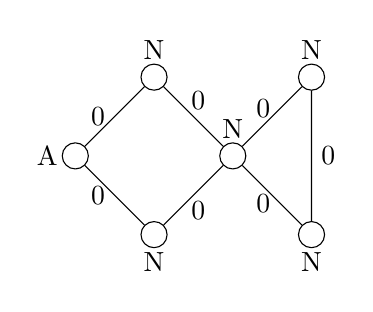
\begin{tikzpicture}
                    \node[draw, circle] (n1) at (0,0) {};
                    \node[draw, circle] (n2) at (1,1) {};
                    \node[draw, circle] (n4) at (1,-1) {};
                    \node[draw, circle] (n3) at (2,0) {};
                    
                    \node[draw, circle] (n5) at (3,-1){};
                    \node[draw, circle] (n6) at (3,1){};
        
                    \draw[-] (n1)--(n2)--(n3)--(n4);
                    \draw[-] (n4)--(n1);
                    \draw[-] (n3)--(n6)--(n5)--(n3);
        
                    \draw[transparent, rounded corners,rotate around={45:(0,-0.5)}, dotted] (0,-0.5) rectangle (2.2,0.3) ;
                    \draw[transparent, rounded corners,rotate around={-45:(0,0.5)}, dotted] (0,0.5) rectangle (2.2,-0.3) ;   
    
                    \draw(-0.1,0) node[left] {A};
                    \draw(1,1.1) node[above] {N};
                    \draw(1,-1.1) node[below] {N};
                    \draw(2,0.1) node[above] {N};
                    \draw(3,1.1) node[above] {N};
                    \draw(3,-1.1) node[below] {N};
    
                    % edge labels
                    \draw(1.35,0.7) node[right] {0};
                    \draw(1.35,-0.7) node[right] {0};
                    \draw(0.5,0.5) node[left] {0};
                    \draw(0.5,-0.5) node[left] {0};
                    \draw(2.6,0.6) node[left] {0};
                    \draw(2.6,-0.6) node[left] {0};
                    \draw(3,0) node[right] {0};
                \end{tikzpicture}
    
            \end{onlyenv}    
            \begin{onlyenv}<2>
                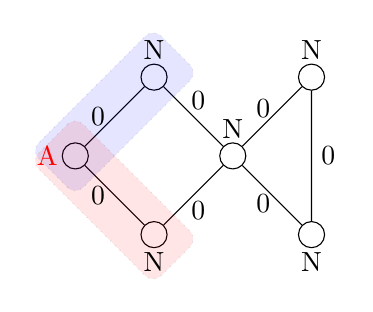
\begin{tikzpicture}
                    \node[draw, circle] (n1) at (0,0) {};
                    \node[draw, circle] (n2) at (1,1) {};
                    \node[draw, circle] (n4) at (1,-1) {};
                    \node[draw, circle] (n3) at (2,0) {};
                    
                    \node[draw, circle] (n5) at (3,-1){};
                    \node[draw, circle] (n6) at (3,1){};
        
                    \draw[-] (n1)--(n2)--(n3)--(n4);
                    \draw[-] (n4)--(n1);
                    \draw[-] (n3)--(n6)--(n5)--(n3);
        
                    \draw[transparent, rounded corners,rotate around={45:(0,-0.5)}, dotted] (0,-0.5) rectangle (2.2,0.3) ;
                    \draw[transparent, rounded corners,rotate around={-45:(0,0.5)}, dotted] (0,0.5) rectangle (2.2,-0.3) ;
                    \draw[fill=blue, opacity=0.1, rounded corners,rotate around={45:(0,-0.5)}, dotted] (0,-0.5) rectangle (2.2,0.3) ;
                    \draw[fill=red,opacity=0.1, rounded corners,rotate around={-45:(0,0.5)}, dotted] (0,0.5) rectangle (2.2,-0.3) ;
           
    
                    \draw(-0.1,0) node[left] {\textcolor{red}{A}};
                    \draw(1,1.1) node[above] {N};
                    \draw(1,-1.1) node[below] {N};
                    \draw(2,0.1) node[above] {N};
                    \draw(3,1.1) node[above] {N};
                    \draw(3,-1.1) node[below] {N};
    
                    % edge labels
                    \draw(1.35,0.7) node[right] {0};
                    \draw(1.35,-0.7) node[right] {0};
                    \draw(0.5,0.5) node[left] {0};
                    \draw(0.5,-0.5) node[left] {0};
                    \draw(2.6,0.6) node[left] {0};
                    \draw(2.6,-0.6) node[left] {0};
                    \draw(3,0) node[right] {0};
                \end{tikzpicture}
            \end{onlyenv}
    
        
    
            \begin{onlyenv}<3>
                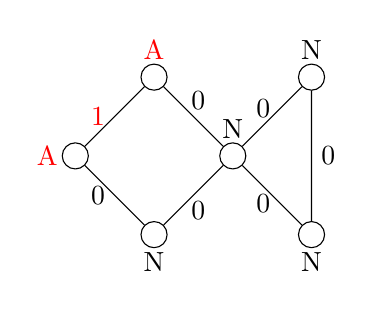
\begin{tikzpicture}
                    \node[draw, circle] (n1) at (0,0) {};
                    \node[draw, circle] (n2) at (1,1) {};
                    \node[draw, circle] (n4) at (1,-1) {};
                    \node[draw, circle] (n3) at (2,0) {};
                    
                    \node[draw, circle] (n5) at (3,-1){};
                    \node[draw, circle] (n6) at (3,1){};
        
                    \draw[-] (n1)--(n2)--(n3)--(n4);
                    \draw[-] (n4)--(n1);
                    \draw[-] (n3)--(n6)--(n5)--(n3);
        
                    \draw[transparent, rounded corners,rotate around={45:(0,-0.5)}, dotted] (0,-0.5) rectangle (2.2,0.3) ;
                    \draw[transparent, rounded corners,rotate around={-45:(0,0.5)}, dotted] (0,0.5) rectangle (2.2,-0.3) ;
    
                    \draw(-0.1,0) node[left] {\textcolor{red}{A}};
                    \draw(1,1.1) node[above] {\textcolor{red}{A}};
                    \draw(1,-1.1) node[below] {N};
                    \draw(2,0.1) node[above] {N};
                    \draw(3,1.1) node[above] {N};
                    \draw(3,-1.1) node[below] {N};
    
                    % edge labels
                    \draw(1.35,0.7) node[right] {0};
                    \draw(1.35,-0.7) node[right] {0};
                    \draw(0.5,0.5) node[left] {\textcolor{red}{1}};
                    \draw(0.5,-0.5) node[left] {0};
                    \draw(2.6,0.6) node[left] {0};
                    \draw(2.6,-0.6) node[left] {0};
                    \draw(3,0) node[right] {0};
                \end{tikzpicture}
                \end{onlyenv}
    
    
                \begin{onlyenv}<4>
                    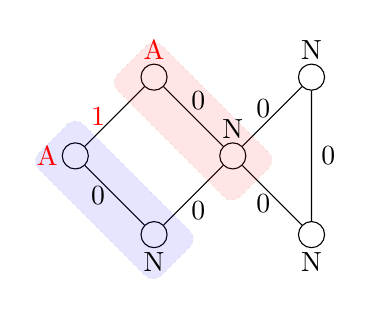
\begin{tikzpicture}
                        \node[draw, circle] (n1) at (0,0) {};
                        \node[draw, circle] (n2) at (1,1) {};
                        \node[draw, circle] (n4) at (1,-1) {};
                        \node[draw, circle] (n3) at (2,0) {};
                        
                        \node[draw, circle] (n5) at (3,-1){};
                        \node[draw, circle] (n6) at (3,1){};
            
                        \draw[-] (n1)--(n2)--(n3)--(n4);
                        \draw[-] (n4)--(n1);
                        \draw[-] (n3)--(n6)--(n5)--(n3);
            
                        \draw[transparent, rounded corners,rotate around={45:(0,-0.5)}, dotted] (0,-0.5) rectangle (2.2,0.3) ;
                        \draw[transparent, rounded corners,rotate around={-45:(0,0.5)}, dotted] (0,0.5) rectangle (2.2,-0.3) ;
                        \draw[fill=red,opacity=0.1, rounded corners, rotate around={-45:(1,1.5)}, dotted] (1,1.5) rectangle (3.2,0.7) ;
                        \draw[fill=blue,opacity=0.1, rounded corners,rotate around={-45:(0,0.5)}, dotted] (0,0.5) rectangle (2.2,-0.3) ;
    
                        \draw(-0.1,0) node[left] {\textcolor{red}{A}};
                        \draw(1,1.1) node[above] {\textcolor{red}{A}};
                        \draw(1,-1.1) node[below] {N};
                        \draw(2,0.1) node[above] {N};
                        \draw(3,1.1) node[above] {N};
                        \draw(3,-1.1) node[below] {N};
    
                        % edge labels
                        \draw(1.35,0.7) node[right] {0};
                        \draw(1.35,-0.7) node[right] {0};
                        \draw(0.5,0.5) node[left] {\textcolor{red}{1}};
                        \draw(0.5,-0.5) node[left] {0};
                        \draw(2.6,0.6) node[left] {0};
                        \draw(2.6,-0.6) node[left] {0};
                        \draw(3,0) node[right] {0};
                    \end{tikzpicture}
                \end{onlyenv}
    %%%%%%%%% ici
             \begin{onlyenv}<5>
                    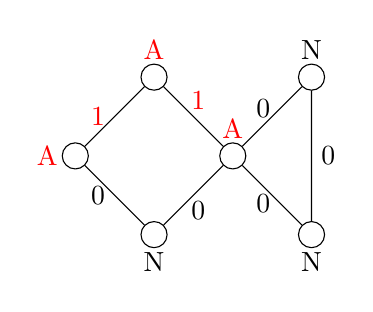
\begin{tikzpicture}
                        \node[draw, circle] (n1) at (0,0) {};
                        \node[draw, circle] (n2) at (1,1) {};
                        \node[draw, circle] (n4) at (1,-1) {};
                        \node[draw, circle] (n3) at (2,0) {};
                        
                        \node[draw, circle] (n5) at (3,-1){};
                        \node[draw, circle] (n6) at (3,1){};
            
                        \draw[-] (n1)--(n2)--(n3)--(n4);
                        \draw[-] (n4)--(n1);
                        \draw[-] (n3)--(n6)--(n5)--(n3);
            
                        \draw[transparent, rounded corners,rotate around={45:(0,-0.5)}, dotted] (0,-0.5) rectangle (2.2,0.3) ;
                        \draw[transparent, rounded corners,rotate around={-45:(0,0.5)}, dotted] (0,0.5) rectangle (2.2,-0.3) ;
    
                        \draw(-0.1,0) node[left] {\textcolor{red}{A}};
                        \draw(1,1.1) node[above] {\textcolor{red}{A}};
                        \draw(1,-1.1) node[below] {N};
                        \draw(2,0.1) node[above] {\textcolor{red}{A}};
                        \draw(3,1.1) node[above] {N};
                        \draw(3,-1.1) node[below] {N};
    
                        % edge labels
                        \draw(1.35,0.7) node[right] {\textcolor{red}{1}};
                        \draw(1.35,-0.7) node[right] {0};
                        \draw(0.5,0.5) node[left] {\textcolor{red}{1}};
                        \draw(0.5,-0.5) node[left] {0};
                        \draw(2.6,0.6) node[left] {0};
                        \draw(2.6,-0.6) node[left] {0};
                        \draw(3,0) node[right] {0};
                    \end{tikzpicture}
                \end{onlyenv}

        \begin{onlyenv}<6>
                    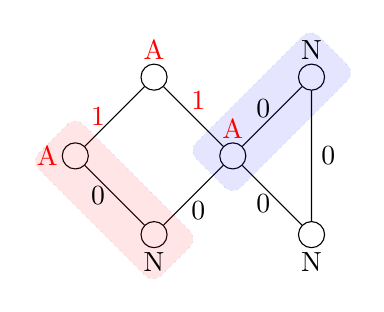
\begin{tikzpicture}
                        \node[draw, circle] (n1) at (0,0) {};
                        \node[draw, circle] (n2) at (1,1) {};
                        \node[draw, circle] (n4) at (1,-1) {};
                        \node[draw, circle] (n3) at (2,0) {};
                        
                        \node[draw, circle] (n5) at (3,-1){};
                        \node[draw, circle] (n6) at (3,1){};
            
                        \draw[-] (n1)--(n2)--(n3)--(n4);
                        \draw[-] (n4)--(n1);
                        \draw[-] (n3)--(n6)--(n5)--(n3);
            
                        \draw[transparent, rounded corners,rotate around={45:(0,-0.5)}, dotted] (0,-0.5) rectangle (2.2,0.3) ;
                        \draw[transparent, rounded corners,rotate around={-45:(0,0.5)}, dotted] (0,0.5) rectangle (2.2,-0.3) ;
                        % \draw[fill=red,opacity=0.1, rounded corners, rotate around={-45:(1,1.5)}, dotted] (1,1.5) rectangle (3.2,0.7) ;
                        \draw[fill=red,opacity=0.1, rounded corners,rotate around={-45:(0,0.5)}, dotted] (0,0.5) rectangle (2.2,-0.3) ;
                        \draw[fill=blue, opacity=0.1, rounded corners,rotate around={45:(2,-0.5)}, dotted] (2,-0.5) rectangle (4.2,0.3) ;

                        \draw(-0.1,0) node[left] {\textcolor{red}{A}};
                        \draw(1,1.1) node[above] {\textcolor{red}{A}};
                        \draw(1,-1.1) node[below] {N};
                        \draw(2,0.1) node[above] {\textcolor{red}{A}};
                        \draw(3,1.1) node[above] {N};
                        \draw(3,-1.1) node[below] {N};
    
                        % edge labels
                        \draw(1.35,0.7) node[right] {\textcolor{red}{1}};
                        \draw(1.35,-0.7) node[right] {0};
                        \draw(0.5,0.5) node[left] {\textcolor{red}{1}};
                        \draw(0.5,-0.5) node[left] {0};
                        \draw(2.6,0.6) node[left] {0};
                        \draw(2.6,-0.6) node[left] {0};
                        \draw(3,0) node[right] {0};
                    \end{tikzpicture}
                \end{onlyenv}

                %%%%%%%%%%%%%%ici

                \begin{onlyenv}<7>
                    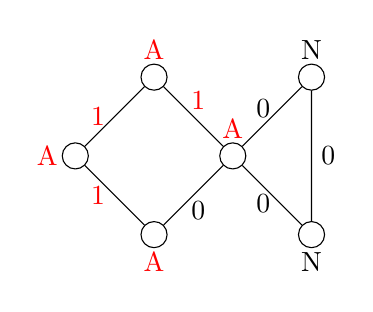
\begin{tikzpicture}
                        \node[draw, circle] (n1) at (0,0) {};
                        \node[draw, circle] (n2) at (1,1) {};
                        \node[draw, circle] (n4) at (1,-1) {};
                        \node[draw, circle] (n3) at (2,0) {};
                        
                        \node[draw, circle] (n5) at (3,-1){};
                        \node[draw, circle] (n6) at (3,1){};
            
                        \draw[-] (n1)--(n2)--(n3)--(n4);
                        \draw[-] (n4)--(n1);
                        \draw[-] (n3)--(n6)--(n5)--(n3);
            
                        \draw[transparent, rounded corners,rotate around={45:(0,-0.5)}, dotted] (0,-0.5) rectangle (2.2,0.3) ;
                        \draw[transparent, rounded corners,rotate around={-45:(0,0.5)}, dotted] (0,0.5) rectangle (2.2,-0.3) ;
    
                        \draw(-0.1,0) node[left] {\textcolor{red}{A}};
                        \draw(1,1.1) node[above] {\textcolor{red}{A}};
                        \draw(1,-1.1) node[below] {\textcolor{red}{A}};
                        \draw(2,0.1) node[above] {\textcolor{red}{A}};
                        \draw(3,1.1) node[above] {N};
                        \draw(3,-1.1) node[below] {N};
    
                        % edge labels
                        \draw(1.35,0.7) node[right] {\textcolor{red}{1}};
                        \draw(1.35,-0.7) node[right] {0};
                        \draw(0.5,0.5) node[left] {\textcolor{red}{1}};
                        \draw(0.5,-0.5) node[left] {\textcolor{red}{1}};
                        \draw(2.6,0.6) node[left] {0};
                        \draw(2.6,-0.6) node[left] {0};
                        \draw(3,0) node[right] {0};
                    \end{tikzpicture}
                \end{onlyenv}
    
                \begin{onlyenv}<8>
                    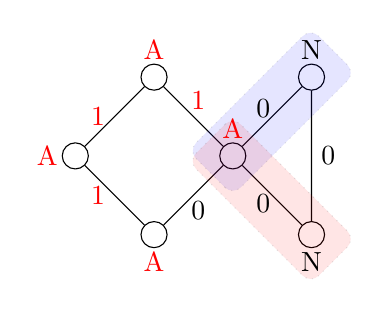
\begin{tikzpicture}
                        \node[draw, circle] (n1) at (0,0) {};
                        \node[draw, circle] (n2) at (1,1) {};
                        \node[draw, circle] (n4) at (1,-1) {};
                        \node[draw, circle] (n3) at (2,0) {};
                        
                        \node[draw, circle] (n5) at (3,-1){};
                        \node[draw, circle] (n6) at (3,1){};
            
                        \draw[-] (n1)--(n2)--(n3)--(n4);
                        \draw[-] (n4)--(n1);
                        \draw[-] (n3)--(n6)--(n5)--(n3);
            
                        \draw[transparent, rounded corners,rotate around={45:(0,-0.5)}, dotted] (0,-0.5) rectangle (2.2,0.3) ;
                        \draw[transparent, rounded corners,rotate around={-45:(0,0.5)}, dotted] (0,0.5) rectangle (2.2,-0.3) ;
                        \draw[fill=blue, opacity=0.1, rounded corners,rotate around={45:(2,-0.5)}, dotted] (2,-0.5) rectangle (4.2,0.3) ;
                        \draw[fill=red, opacity=0.1, rounded corners,rotate around={-45:(2,0.5)}, dotted] (2,0.5) rectangle (4.2,-0.3) ;
                     
                        \draw(-0.1,0) node[left] {\textcolor{red}{A}};
                        \draw(1,1.1) node[above] {\textcolor{red}{A}};
                        \draw(1,-1.1) node[below] {\textcolor{red}{A}};
                        \draw(2,0.1) node[above] {\textcolor{red}{A}};
                        \draw(3,1.1) node[above] {N};
                        \draw(3,-1.1) node[below] {N};
    
                        % edge labels
                        \draw(1.35,0.7) node[right] {\textcolor{red}{1}};
                        \draw(1.35,-0.7) node[right] {0};
                        \draw(0.5,0.5) node[left] {\textcolor{red}{1}};
                        \draw(0.5,-0.5) node[left] {\textcolor{red}{1}};
                        \draw(2.6,0.6) node[left] {0};
                        \draw(2.6,-0.6) node[left] {0};
                        \draw(3,0) node[right] {0};
                    \end{tikzpicture}
                \end{onlyenv}
    
                \begin{onlyenv}<9>
                    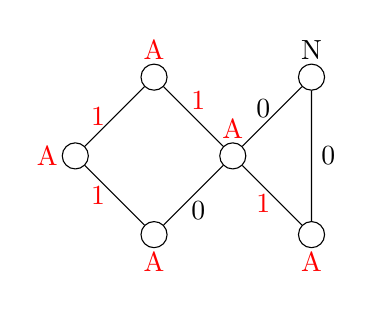
\begin{tikzpicture}
                        \node[draw, circle] (n1) at (0,0) {};
                        \node[draw, circle] (n2) at (1,1) {};
                        \node[draw, circle] (n4) at (1,-1) {};
                        \node[draw, circle] (n3) at (2,0) {};
                        
                        \node[draw, circle] (n5) at (3,-1){};
                        \node[draw, circle] (n6) at (3,1){};
            
                        \draw[-] (n1)--(n2)--(n3)--(n4);
                        \draw[-] (n4)--(n1);
                        \draw[-] (n3)--(n6)--(n5)--(n3);
            
                        \draw[transparent, rounded corners,rotate around={45:(0,-0.5)}, dotted] (0,-0.5) rectangle (2.2,0.3) ;
                        \draw[transparent, rounded corners,rotate around={-45:(0,0.5)}, dotted] (0,0.5) rectangle (2.2,-0.3) ;
              
                        \draw(-0.1,0) node[left] {\textcolor{red}{A}};
                        \draw(1,1.1) node[above] {\textcolor{red}{A}};
                        \draw(1,-1.1) node[below] {\textcolor{red}{A}};
                        \draw(2,0.1) node[above] {\textcolor{red}{A}};
                        \draw(3,1.1) node[above] {N};
                        \draw(3,-1.1) node[below] {\textcolor{red}{A}};
    
                        % edge labels
                        \draw(1.35,0.7) node[right] {\textcolor{red}{1}};
                        \draw(1.35,-0.7) node[right] {0};
                        \draw(0.5,0.5) node[left] {\textcolor{red}{1}};
                        \draw(0.5,-0.5) node[left] {\textcolor{red}{1}};
                        \draw(2.6,0.6) node[left] {0};
                        \draw(2.6,-0.6) node[left] {\textcolor{red}{1}};
                        \draw(3,0) node[right] {0};
                    \end{tikzpicture}
                \end{onlyenv}
    
                \begin{onlyenv}<10>
                    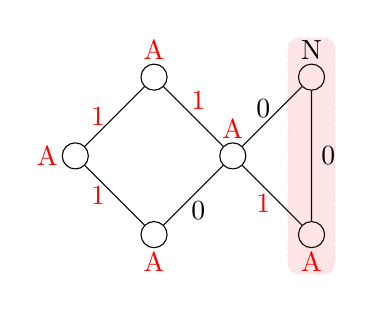
\begin{tikzpicture}
                        \node[draw, circle] (n1) at (0,0) {};
                        \node[draw, circle] (n2) at (1,1) {};
                        \node[draw, circle] (n4) at (1,-1) {};
                        \node[draw, circle] (n3) at (2,0) {};
                        
                        \node[draw, circle] (n5) at (3,-1){};
                        \node[draw, circle] (n6) at (3,1){};
            
                        \draw[-] (n1)--(n2)--(n3)--(n4);
                        \draw[-] (n4)--(n1);
                        \draw[-] (n3)--(n6)--(n5)--(n3);
            
                        \draw[transparent, rounded corners,rotate around={45:(0,-0.5)}, dotted] (0,-0.5) rectangle (2.2,0.3) ;
                        \draw[transparent, rounded corners,rotate around={-45:(0,0.5)}, dotted] (0,0.5) rectangle (2.2,-0.3) ;
                        \draw[fill=red,opacity=0.1 , rounded corners, dotted] (2.7,-1.5) rectangle (3.3,1.5) ;  
                        \draw(-0.1,0) node[left] {\textcolor{red}{A}};
                        \draw(1,1.1) node[above] {\textcolor{red}{A}};
                        \draw(1,-1.1) node[below] {\textcolor{red}{A}};
                        \draw(2,0.1) node[above] {\textcolor{red}{A}};
                        \draw(3,1.1) node[above] {N};
                        \draw(3,-1.1) node[below] {\textcolor{red}{A}};
     
                        % edge labels
                        \draw(1.35,0.7) node[right] {\textcolor{red}{1}};
                        \draw(1.35,-0.7) node[right] {0};
                        \draw(0.5,0.5) node[left] {\textcolor{red}{1}};
                        \draw(0.5,-0.5) node[left] {\textcolor{red}{1}};
                        \draw(2.6,0.6) node[left] {0};
                        \draw(2.6,-0.6) node[left] {\textcolor{red}{1}};
                        \draw(3,0) node[right] {0};
                    \end{tikzpicture}
                \end{onlyenv}
    
                \begin{onlyenv}<11>
                    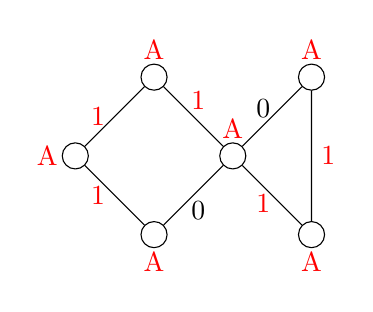
\begin{tikzpicture}
                        \node[draw, circle] (n1) at (0,0) {};
                        \node[draw, circle] (n2) at (1,1) {};
                        \node[draw, circle] (n4) at (1,-1) {};
                        \node[draw, circle] (n3) at (2,0) {};
                        
                        \node[draw, circle] (n5) at (3,-1){};
                        \node[draw, circle] (n6) at (3,1){};
            
                        \draw[-] (n1)--(n2)--(n3)--(n4);
                        \draw[-] (n4)--(n1);
                        \draw[-] (n3)--(n6)--(n5)--(n3);
            
                        \draw[transparent, rounded corners,rotate around={45:(0,-0.5)}, dotted] (0,-0.5) rectangle (2.2,0.3) ;
                        \draw[transparent, rounded corners,rotate around={-45:(0,0.5)}, dotted] (0,0.5) rectangle (2.2,-0.3) ;
                        \draw(-0.1,0) node[left] {\textcolor{red}{A}};
                        \draw(1,1.1) node[above] {\textcolor{red}{A}};
                        \draw(1,-1.1) node[below] {\textcolor{red}{A}};
                        \draw(2,0.1) node[above] {\textcolor{red}{A}};
                        \draw(3,1.1) node[above] {\textcolor{red}{A}};
                        \draw(3,-1.1) node[below] {\textcolor{red}{A}};
    
                        % edge labels
                        \draw(1.35,0.7) node[right] {\textcolor{red}{1}};
                        \draw(1.35,-0.7) node[right] {0};
                        \draw(0.5,0.5) node[left] {\textcolor{red}{1}};
                        \draw(0.5,-0.5) node[left] {\textcolor{red}{1}};
                        \draw(2.6,0.6) node[left] {0};
                        \draw(2.6,-0.6) node[left] {\textcolor{red}{1}};
                        \draw(3,0) node[right] {\textcolor{red}{1}};
                    \end{tikzpicture}
                \end{onlyenv}
                \begin{onlyenv}<12>
                    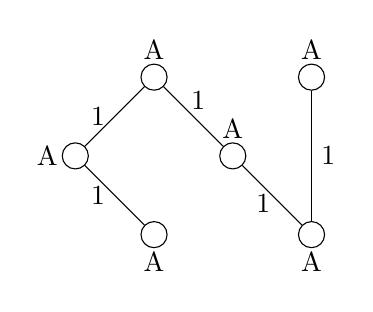
\begin{tikzpicture}
                        \node[draw, circle] (n1) at (0,0) {};
                        \node[draw, circle] (n2) at (1,1) {};
                        \node[draw, circle] (n4) at (1,-1) {};
                        \node[draw, circle] (n3) at (2,0) {};
                        
                        \node[draw, circle] (n5) at (3,-1){};
                        \node[draw, circle] (n6) at (3,1){};
            
                        \draw[-] (n1)--(n2);
                        \draw[-] (n2)--(n3);
                        % \draw[-] (n3)--(n4);
                        \draw[-] (n4)--(n1);
                        % \draw[-] (n3)--(n6);
                        \draw[-] (n6)--(n5);
                        \draw[-] (n5)--(n3);
            
                        \draw[transparent, rounded corners,rotate around={45:(0,-0.5)}, dotted] (0,-0.5) rectangle (2.2,0.3) ;
                        \draw[transparent, rounded corners,rotate around={-45:(0,0.5)}, dotted] (0,0.5) rectangle (2.2,-0.3) ;
                        \draw(-0.1,0) node[left] {A};
                        \draw(1,1.1) node[above] {A};
                        \draw(1,-1.1) node[below] {A};
                        \draw(2,0.1) node[above] {A};
                        \draw(3,1.1) node[above] {A};
                        \draw(3,-1.1) node[below] {A};
    
                        % edge labels
                        \draw(1.35,0.7) node[right] {1};
                        \draw(0.5,0.5) node[left] {1};
                        \draw(0.5,-0.5) node[left] {1};
                        \draw(2.6,-0.6) node[left] {1};
                        \draw(3,0) node[right] {1};
                    \end{tikzpicture}
                    % \begin{tikzpicture}
                    %     \node[draw, circle] (n1) at (0,0) {};
                    %     \node[draw, circle] (n2) at (1,1) {};
                    %     \node[draw, circle] (n4) at (1,-1) {};
                    %     \node[draw, circle] (n3) at (2,0) {};
                        
                    %     \node[draw, circle] (n5) at (3,-1){};
                    %     \node[draw, circle] (n6) at (3,1){};
            
                    %     \draw[-] (n1)--(n2);
                    %     \draw[-] (n2)--(n3);
                    %     % \draw[-] (n3)--(n4);
                    %     \draw[-] (n4)--(n1);
                    %     % \draw[-] (n3)--(n6);
                    %     \draw[-] (n6)--(n5);
                    %     \draw[-] (n5)--(n3);
            
                    %     \draw[transparent, rounded corners,rotate around={45:(0,-0.5)}, dotted] (0,-0.5) rectangle (2.2,0.3) ;
                    %     \draw[transparent, rounded corners,rotate around={-45:(0,0.5)}, dotted] (0,0.5) rectangle (2.2,-0.3) ;
                    % \end{tikzpicture}
                \end{onlyenv}
            \end{overlayarea}

\vspace{4mm}

\end{frame}
\subsection{Termination via Translation to Term Rewriting Systems}
\begin{frame}
   \tableofcontents[currentsubsection]
\end{frame}
\begin{frame}{Term Rewriting Systems (TRS)}
	\begin{itemize}
		\item Rule based term transformation\\
		\item Example of a TRS:\\
			\begin{align*}
				r_1:& \textcolor{red}{f}(x)  \longrightarrow \textcolor{red}{g}(x)\\
				r_2:& \textcolor{red}{a}     \longrightarrow \textcolor{red}{b}
			\end{align*}\\
		\item Example of an execution:\\
			$f(a) \overset{\alert{r_1}}{\longrightarrow} g(a) \overset{\alert{r_2}}{\longrightarrow} g(b)$
        \item Can we make use existing advanced termination techniques for TRS?
    
    \end{itemize}
\end{frame}
 
\begin{frame}{Translation into TRS with AC Symbols}
    \begin{adjustwidth}{-1.5cm}{0cm}
         \begin{description}
            \item Example: 
            \begin{center} 
                \resizebox{0.7\textwidth}{!}{
                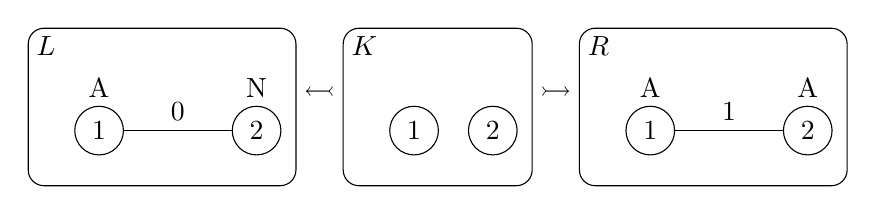
\begin{tikzpicture}
                    \graphbox{$L$}{0mm}{0mm}{34mm}{20mm}{2mm}{-5mm}{
                        \coordinate (o) at (0mm,-8mm); 
                        \node[draw,circle] (l1) at ($(o)+(-10mm,0mm)$) {1};
                        \node[draw,circle] (l2) at ($(l1)+(2,0)$) {2};
                        \draw ($(o)+(-10mm,3mm)$) node[above] {A};
                        \draw ($(l1)+(2,3mm)$) node[above] {N};
                        \draw[-] (l1) -- (l2) node[midway,above] {0};
                    }     
                    \graphbox{$K$}{40mm}{0mm}{24mm}{20mm}{2mm}{-5mm}{
                        \coordinate (o) at (5mm,-8mm); 
                        \node[draw,circle] (l1) at ($(o)+(-10mm,0mm)$) {1};
                        \node[draw,circle] (l2) at ($(l1)+(1,0)$) {2};
                        % \node[draw,circle] (l3) at ($(l1) + (1,0)$) {$\ $};
                        % \draw[->] (l1) -- (l3) node[midway,above] {a};
                        % \draw[->] (l3) -- (l2) node[midway,above] {a};
                    }    
                    \graphbox{$R$}{70mm}{0mm}{34mm}{20mm}{2mm}{-5mm}{
                            \coordinate (o) at (0mm,-8mm); 
                        \node[draw,circle] (l1) at ($(o)+(-10mm,0mm)$) {1};
                        \node[draw,circle] (l2) at ($(l1)+(2,0)$) {2};
                        \draw ($(o)+(-10mm,3mm)$) node[above] {A};
                        \draw ($(l1)+(2,3mm)$) node[above] {A};
                        \draw[-] (l1) -- (l2) node[midway,above] {1};
                    }    
                    \node () at (37mm,-8mm) {$\leftarrowtail$};
                    \node () at (67mm,-8mm) {$\rightarrowtail$};
                    % \draw[>->] (51mm,2mm) -- (52mm,3mm);
                \end{tikzpicture}
                }
            \end{center}
            \item Translation :  

            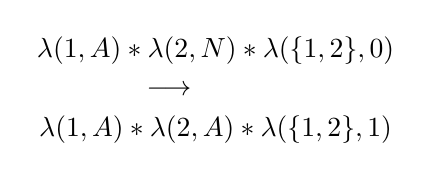
\begin{tikzpicture}
            \draw (0,0) node{$\lambda(1,A)* 
                        \lambda(2,N) * \lambda(\{1,2\},0)$};           

            \draw (-1,-0.5) node[right] {$\longrightarrow$};
            
            \draw (0,-1) node{$\lambda(1,A)* 
                \lambda(2,A) * \lambda(\{1,2\},1)$};

            \end{tikzpicture} 
        
            \item \alert{Preservation of the termination property}:
            \tikz {
                \node (a) at (0,0) {A};
                \node (grs) at (3,0) {GRS};
                \node (trs) at (6,0) {TRS};
                \node (pgrs) at (3,2) {GRS terminates};
                \node (ptrs) at (6,2) {TRS terminates};
                \node (pa) at (0,2) {A terminates};
                \draw[-latex] (a)--(grs);
                \draw[-latex] (grs) --(trs);
                \draw[-latex] (trs)--(ptrs);
                \draw[-latex] (ptrs)--(pgrs);
                \draw[-latex] (pgrs) --(pa);
                \draw[-latex,dashed] (grs)--(pgrs);
                \draw[-latex,dashed,red] (a)--(pa); 
            }
        % \item<1-> Problème: difficile de modéliser un algorithme avec GRS
        % \item<1-> Question: existe-il une façon plus facile pour modéliser les algorithmes distribués
    \end{description}
\end{adjustwidth}
\end{frame}

\begin{frame}{Other Translations}
    Translation into 
    \begin{itemize}
        \item Normalized Term Rewriting Systems (NTRS)
        \item Hierarchical Term Rewriting Systems (HTRS) with innermost strategy
        \item two others translations
            %   \begin{itemize}
            %     \item Graph and graph relabeling rules encoded in a term $\approx$ State Machine
            %     \item Term rewriting rules $\approx$ Transitions
            %   \end{itemize} 
    \end{itemize} 
    Limitations 
    \begin{itemize}
        \item Termination techniques for Term Rewriting Systems rely heavily on the \alert{tree structure of terms}
        \item Graph has no tree structure
        \item New difficulties introduced by translation
    \end{itemize}
    % Except two techniques and they have been adapted to Graph Rewriting Systems
    Termination techniques for DPO Graph Rewriting Systems
\end{frame}
 

\subsection{Termination using Weighted Type Graphs}
\begin{frame}
    \tableofcontents[currentsubsection]
\end{frame}

\begin{frame}{Well-founded semirings}
    A mathematical structure $(S, \oplus, \otimes, 0, 1, \prec, \preceq)$ 
    \begin{itemize}
        \item $\otimes$, $\oplus$ : binary operations
        \item $0$, $1$ : neutral elements for $\oplus$, $\otimes$
        \item $\prec, \preceq$ : orders
        \item $\prec/\preceq$ : \alert{well-founded}
        \item satisfies some conditions
    \end{itemize}

    Examples:
    \begin{itemize}
        \item The natural arithmetic semiring $(\mathbb{N},+,*,0,1,<,\leq)$
        \item The natural tropical semiring: $(\mathbb{N} \cup \{+\infty\},\min,+,+\infty, 0,<,\leq)$
        \item The natural arctic semiring: $(\mathbb{N} \cup \{-\infty\},\max,+,-\infty, 0,<,\leq)$
    \end{itemize}

\end{frame}


\begin{frame}{Termination using Weighted Type Graphs}
  \begin{description}
    \item[Termination of]

    \begin{center} 
                \resizebox{0.7\textwidth}{!}{
                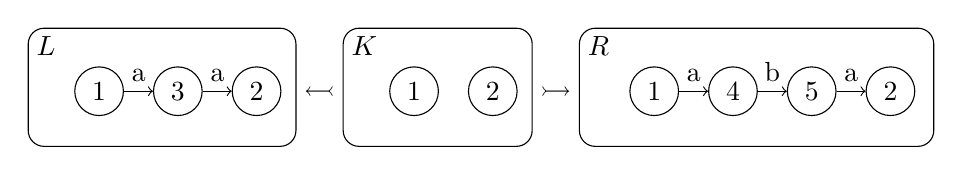
\begin{tikzpicture}
                    \graphbox{$L$}{0mm}{0mm}{34mm}{15mm}{2mm}{-5mm}{
                        \coordinate (o) at (0mm,-3mm); 
                        \node[draw,circle] (l1) at ($(o)+(-10mm,0mm)$) {1};
                        \node[draw,circle] (l2) at ($(l1)+(2,0)$) {2};
                        \node[draw,circle] (l3) at ($(l1) + (1,0)$) {3};
                        \draw[->] (l1) -- (l3) node[midway,above] {a};
                        \draw[->] (l3) -- (l2) node[midway,above] {a};
                    }     
                    \graphbox{$K$}{40mm}{0mm}{24mm}{15mm}{2mm}{-5mm}{
                        \coordinate (o) at (5mm,-3mm); 
                        \node[draw,circle] (l1) at ($(o)+(-10mm,0mm)$) {1};
                        \node[draw,circle] (l2) at ($(l1)+(1,0)$) {2};
                        % \node[draw,circle] (l3) at ($(l1) + (1,0)$) {$\ $};
                        % \draw[->] (l1) -- (l3) node[midway,above] {a};
                        % \draw[->] (l3) -- (l2) node[midway,above] {a};
                    }    
                    \graphbox{$R$}{70mm}{0mm}{45mm}{15mm}{2mm}{-5mm}{
                        \coordinate (o) at (-5mm,-3mm); 
                        \node[draw,circle] (l1) at ($(o)+(-10mm,0mm)$) {1};
                        \node[draw,circle] (l2) at ($(l1)+(3,0)$) {2};
                        \node[draw,circle] (l3) at ($(l1) + (1,0)$) {4};
                        \node[draw,circle] (l4) at ($(l1) + (2,0)$) {5};
                        \draw[->] (l1) -- (l3) node[midway,above] {a};
                        \draw[->] (l3) -- (l4) node[midway,above] {b};
                        \draw[->] (l4) -- (l2) node[midway,above] {a};
                    }    
                    \node () at (37mm,-8mm) {$\leftarrowtail$};
                    \node () at (67mm,-8mm) {$\rightarrowtail$};
                    % \draw[>->] (51mm,2mm) -- (52mm,3mm);
                \end{tikzpicture}
                }
            \end{center}
    \item[by the weighted type graphs over the natural arithmetic semiring.]
    %  finite graphs with weighted edges
  \end{description}
    \begin{center}
        \resizebox{0.3\textwidth}{!}{ 
                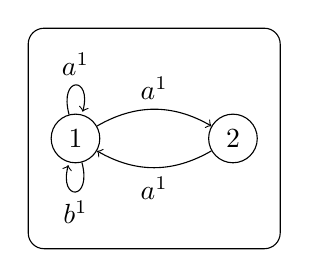
\begin{tikzpicture}
                    \graphbox{}{0mm}{0mm}{32mm}{28mm}{-10mm}{-14mm}{
                        \node[draw,circle] (1) at (0,0) {1};
                        \node[draw,circle] (2) at (2,0) {2};
                        \draw[->] (1) edge[loop above] node[midway, above] {$a^{1}$} (1) ;
                        \draw[->] (1) edge[loop below] node[midway, below] {$b^{1}$} (1) ;
                        \draw[->] (1) edge[bend left] node[midway, above] {$a^{1}$}  (2)  ;
                        \draw[->] (2) edge[bend left] node[midway, below] {$a^{1}$} (1)   ;
                    }
                \end{tikzpicture}
        }
    \end{center}
    % satisfying some conditions expressed as existential Presburger/Peano arithmetic formula
  \begin{description}
    % \item[Witness of termination if] a first-order existential formula in Presburger or Peano arithmetic is satisfied
    \item[Existence of suitable weighted type graphs:]\ \\
        \begin{adjustwidth}{-2cm}{0cm} 
            \begin{itemize}
                \item undecidable in general
            \end{itemize}
        \end{adjustwidth}
  \end{description}
\end{frame}

\begin{frame}{Practical Solution, its Limitation, and our Solution}
    $\Sigma$ : finite set of labels 
  \begin{description}
    \item[Searching a weighted type graph] with\\
    \begin{itemize}
    \item $k \in \mathbb{N}$ nodes
    \item no parallel edges with the same label
    \end{itemize} 
    \begin{adjustwidth}{-2cm}{0cm}
        \begin{enumerate}
            % \item Construct a graph \( T \) with
            %     \begin{itemize}
            %       \item an edge $s \overset{l}{\to} t$ for every pair of nodes \( s, t\) and label \( l\)
            %       \item the number of arrows in $T$ denoted by \( n \)
            %     \end{itemize}
            \item Decide if $s \overset{l}{\to} t$ exists for every pair of nodes \( s, t\) and label \( l\)
            \item Assign a weight to every existing edge
            \item Check if the weighted type graph satisfy requirements
            % weights satisfy the conditions expressed as an existential first-order formula in Presburger or Peano arithmetic
        \end{enumerate}
    \end{adjustwidth}
\end{description}

\begin{description}
    \item[Complexity] $O(2^{2n})$ or undecidable
         \begin{itemize}
            \item $n = k^2 \cdot |\Sigma|$
         \end{itemize}
    \item[\alert{Solution:}] weighted type graph over real numbers
    \item[\alert{Result:}] $O(2^{2n}) \Rightarrow O(2^n)$ or $\text{undecidable} \Rightarrow \text{decidable}$
  \end{description}
\end{frame}

\begin{frame}{Intuition}
    \begin{description}
        \item[Rewriting system $\mathcal{R}$ defines binary rewriting relation $\Rightarrow_{\mathcal{R}}$] 
        \item[A weighted type graph over natural numbers defines ]\ \\ 
        %  \begin{adjustwidth}{-2cm}{0cm}
            \begin{itemize}
                \item a homomorphism $h : (\textbf{Graph}, \Rightarrow_{\mathcal{R}}) \to (\mathbb{N},<)$
            \end{itemize}
        %  \end{adjustwidth} 
        \item[Codomain of $h$ can be $(\mathbb{R},<)$ if ]\ \\
        %  \begin{adjustwidth}{-2cm}{0cm}
          \begin{itemize}
            \item there is $\delta > 0$
            \item for all rewriting steps $G \Rightarrow H$: 
            % \begin{adjustwidth}{-0.5cm}{0cm}
                  \begin{itemize}
                    \item $h(G) \geq 0$ 
                    \item $h(G) - h(H) \geq \delta$
                  \end{itemize}
            % \end{adjustwidth}
          \end{itemize}
        % \end{adjustwidth}
    \end{description}
\end{frame}

\begin{frame}{Non-well-founded Semirings}
    \textcolor{red}{Non-well-founded} semiring $(S, \oplus, \otimes, 0, 1,\prec,\preceq, \mu)$
    \begin{itemize}
        \item $\otimes$, $\oplus$ : binary operations
        \item $0$, $1$ : neutral elements for $\oplus$, $\otimes$
        \item $\prec, \preceq$ : orders
        \item \textcolor{blue}{homomorphism} $\mu : (S, \prec) \to ( \overline{\mathbb{R}}, < )$
        \item $\prec$, $\otimes$, $\oplus$ satisfy some conditions
    \end{itemize}

    \textcolor{red}{Well-founded} semiring $(S, \oplus, \otimes, 0, 1, \prec, \preceq)$ 
    \begin{itemize}
        \item $\otimes$, $\oplus$ : binary operations
        \item $0$, $1$ : neutral elements for $\oplus$, $\otimes$
        \item $\prec, \preceq$ : orders
        \item $\prec/\preceq$ : \textcolor{blue}{well-founded}
        \item $\prec,\preceq$, $\otimes$, $\oplus$ satisfy some conditions
    \end{itemize}
\end{frame}

\begin{frame}
        The tropical, arctic, and arithmetic semirings are instances of non-well-founded semirings.
    \begin{itemize}
        \item  The natural tropical semiring: $\mathfrak{T} = (\mathbb{N} \cup \{+\infty\},\min,+,+\infty, 0, < , \alert{\operatorname{id}_{\mathbb{N} \cup \{+\infty\}}})$
        \item The natural arctic semiring: $\mathfrak{A} = (\mathbb{N} \cup \{-\infty\},\max,+,-\infty, 0,<, \alert{\operatorname{id}_{\mathbb{N} \cup \{-\infty\}}})$ 
        \item The natural arithmetic semiring $\mathfrak{N} = (\mathbb{N},+,*,0,1,<, \alert{\operatorname{id}_\mathbb{N}})$
    \end{itemize}
\end{frame}

\begin{frame}{Termination result}
    \begin{theorem}[Termination of DPO rewriting system] 
    Let $\varphi$ be a DPO rewriting rule, $T$ a finite weighted type graph over 
    one of our non-well-founded semirings over real numbers such that

     \begin{enumerate}
        \item edge weights are positive real numbers
        % \item\label{thm1:hyp4} $\{s \in S\mid 1_S \leq s \neq 0_S\} \subseteq \mathbb{R}_{>0}$ 
        % \item\label{thm1:hyp4} for all $x \in S$, if $ 1_S \preceq x \neq 0_S$ then $\mu(x) \geq \mu(1_S)$ and $\mu(x) \in \mathbb{R}$,
        % \item for all $x \in S$, if $ 1_S \preceq x \neq 0_S$ then $\mu(x) \geq \mu(1_S)$ and $\mu(x) \in \mathbb{R}$, and
        \item the rule satisfies some conditions.
        % for every rule $\rho \in (\mathcal{A }\cup \mathcal{B })$ and every double pushout diagram  
        % $\Delta \in \mathfrak{F}(\rho)$ 
        % \begin{itemize}
        %     \item \(\operatorname{left}(\Delta)\) is weighable with \(\mathcal{T}\),
        %     \item \(\operatorname{right}(\Delta)\) is bounded above by \(\mathcal{T}\). 
        % \end{itemize}
        \item there is $\delta >0$ such that: for all rewriting step $G \Rightarrow H$, we have $w(G) - w(H) \succeq \delta$
    \end{enumerate}
    then $\varphi$ terminates. 
\end{theorem} 
\end{frame}


\begin{frame}{Example with Non-well-founded Semirings}
  \begin{description}
    \item[Termination of]

    \begin{center} 
                \resizebox{0.7\textwidth}{!}{
                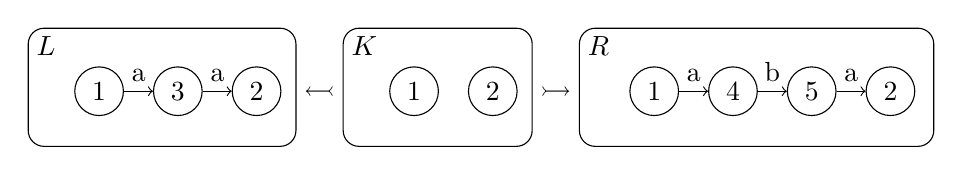
\begin{tikzpicture}
                    \graphbox{$L$}{0mm}{0mm}{34mm}{15mm}{2mm}{-5mm}{
                        \coordinate (o) at (0mm,-3mm); 
                        \node[draw,circle] (l1) at ($(o)+(-10mm,0mm)$) {1};
                        \node[draw,circle] (l2) at ($(l1)+(2,0)$) {2};
                        \node[draw,circle] (l3) at ($(l1) + (1,0)$) {3};
                        \draw[->] (l1) -- (l3) node[midway,above] {a};
                        \draw[->] (l3) -- (l2) node[midway,above] {a};
                    }     
                    \graphbox{$K$}{40mm}{0mm}{24mm}{15mm}{2mm}{-5mm}{
                        \coordinate (o) at (5mm,-3mm); 
                        \node[draw,circle] (l1) at ($(o)+(-10mm,0mm)$) {1};
                        \node[draw,circle] (l2) at ($(l1)+(1,0)$) {2};
                        % \node[draw,circle] (l3) at ($(l1) + (1,0)$) {$\ $};
                        % \draw[->] (l1) -- (l3) node[midway,above] {a};
                        % \draw[->] (l3) -- (l2) node[midway,above] {a};
                    }    
                    \graphbox{$R$}{70mm}{0mm}{45mm}{15mm}{2mm}{-5mm}{
                        \coordinate (o) at (-5mm,-3mm); 
                        \node[draw,circle] (l1) at ($(o)+(-10mm,0mm)$) {1};
                        \node[draw,circle] (l2) at ($(l1)+(3,0)$) {2};
                        \node[draw,circle] (l3) at ($(l1) + (1,0)$) {4};
                        \node[draw,circle] (l4) at ($(l1) + (2,0)$) {5};
                        \draw[->] (l1) -- (l3) node[midway,above] {a};
                        \draw[->] (l3) -- (l4) node[midway,above] {b};
                        \draw[->] (l4) -- (l2) node[midway,above] {a};
                    }    
                    \node () at (37mm,-8mm) {$\leftarrowtail$};
                    \node () at (67mm,-8mm) {$\rightarrowtail$};
                    % \draw[>->] (51mm,2mm) -- (52mm,3mm);
                \end{tikzpicture}
                }
            \end{center}
    \item[by the weighted type graphs over the real arithmetic semiring.]
    %  finite graphs with weighted edges
  \end{description}
    \begin{center}
        \resizebox{0.3\textwidth}{!}{ 
                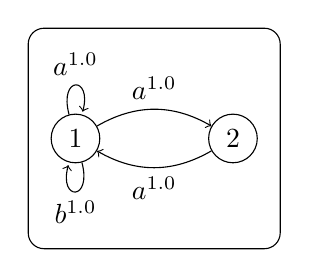
\begin{tikzpicture}
                    \graphbox{}{0mm}{0mm}{32mm}{28mm}{-10mm}{-14mm}{
                        \node[draw,circle] (1) at (0,0) {1};
                        \node[draw,circle] (2) at (2,0) {2};
                        \draw[->] (1) edge[loop above] node[midway, above] {$a^{1.0}$} (1) ;
                        \draw[->] (1) edge[loop below] node[midway, below] {$b^{1.0}$} (1) ;
                        \draw[->] (1) edge[bend left] node[midway, above] {$a^{1.0}$}  (2)  ;
                        \draw[->] (2) edge[bend left] node[midway, below] {$a^{1.0}$} (1)   ;
                    }
                \end{tikzpicture}
        }
    \end{center}

    For every rewriting step $G \Rightarrow H$, we have $w(G) - w(H) \geq 1.0$.
    % satisfying some conditions expressed as existential Presburger/Peano arithmetic formula
%   \begin{description}
%     % \item[Witness of termination if] a first-order existential formula in Presburger or Peano arithmetic is satisfied
%   \end{description}
\end{frame}

% \begin{frame}{Strenghs and limitations}
%   \begin{description}
%     \item[Strenghs:]
%       \begin{itemize}
%         \item Lower Complexity
%         \item No need of user-specified maximum weight
%         % [ ] 
%       \end{itemize}
%     \item[Limitations:] 
%     The reduced complexity is still high, therefore using well founded semirings allows to impose maximum weights in order to reduced the search space
%   \end{description}
% \end{frame}

\begin{frame}{Contribution}
  \begin{description}
    \item[Extension of the existing approach to real numbers]
    \item[Automated Termination Prover:] LyonParallel
       \begin{adjustwidth}{-2cm}{0cm}
            \begin{itemize}
            \item our approach
            \item previous approach
            \item parallel execution
            \item cooperation
            \item more user-friendly for non-experts than existing tools
            \item OCaml
            \end{itemize} 
       \end{adjustwidth}
    \item[Accepted for publication] \ \\

    \begin{adjustwidth}{-2cm}{0cm}
            \begin{itemize}
            \item International Workshop on Graph Computation Models 2025
            \end{itemize} 
       \end{adjustwidth}
  \end{description}
\end{frame}


\subsection{Termination using Subgraph Counting}
\begin{frame}
   \tableofcontents[currentsubsection]
\end{frame}
\begin{frame}{Limitation of Existing Techniques}

    Injective DPO graph rewriting rule:
    \begin{center}
        \resizebox{0.8\textwidth}{!}{
            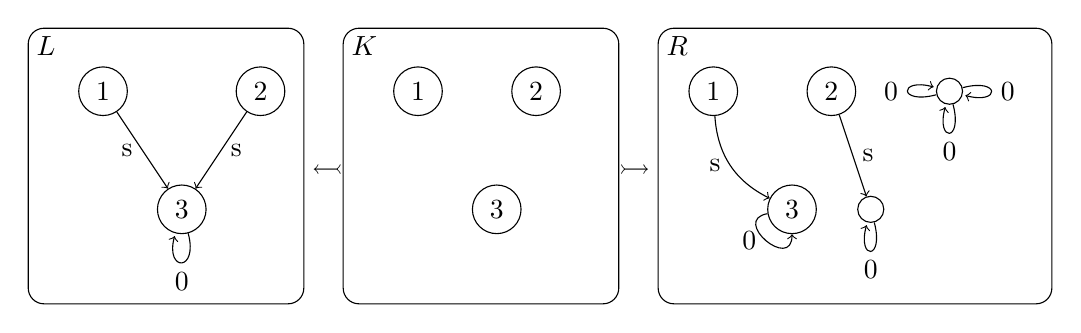
\begin{tikzpicture}
                \graphbox{$L$}{0mm}{0mm}{35mm}{35mm}{2mm}{-5mm}{
                    \coordinate (delta) at (0,-18mm);
                    \node[draw,circle] (l1) at ($(delta) + (-1,1.5)$) {1};
                    \node[draw,circle] (l2) at ($(delta) + (1,1.5)$) {2};
                    \node[draw,circle] (l3) at ($(delta) + (0,0)$) {3};
                    \draw[->] (l1) -- (l3) node[midway,left] {s};
                    \draw[->] (l2) -- (l3) node[midway,right] {s};
                    \draw[->] (l3) edge [loop below] node {0} (l3);
                }
                    \graphbox{$K$}{40mm}{0mm}{35mm}{35mm}{2mm}{-5mm}{
                        \coordinate (delta) at (0,-18mm);
                        \coordinate (interfaceorigin) at ($(delta) +(5,0)$);
                        \node[draw,circle] (r1) at ($(delta) +(-1,1.5)$) {1};
                        \node[draw,circle] (r2) at ($(delta) +(0.5,1.5)$) {2};
                        \node[draw,circle] (r3) at ($(delta) + (0,0)$) {3};
                        % \draw[->] (r1) -- (r3) node[midway,left] {s};
                        % \draw[->] (r3) edge [loop below] node {0} (r3);
                    } 
                    \node () at (38mm,-18mm) {$\leftarrowtail$};
                    \node () at (77mm,-18mm) {$\rightarrowtail$};
                \graphbox{$R$}{80mm}{0mm}{50mm}{35mm}{2mm}{-5mm}{
                    \coordinate (delta) at (-10mm,-18mm);
                    \node[draw,circle] (r1) at ($(delta) + (-1,1.5)$) {1};
                    \node[draw,circle] (r2) at ($(delta) + (0.5,1.5)$) {2};
                    \node[draw,circle] (r3) at ($(delta) + (0,0)$) {3};
                    \node[draw,circle] (r4) at ($(delta) + (1,0)$) {};
                    \draw[->] (r1) edge[bend right] node[midway,left] {s} (r3) ;
                    \draw[->] (r2) -- (r4) node[midway,right] {s};
                    \draw[->] (r4) edge [loop below] node {0} (r4);
                    
                    \draw[->] (r3) edge [out=190,in=270,looseness=3] node[midway,left] {0} (r3);
                    \node[draw,circle] (r5) at ($(r2) + (1.5,0)$) {};
                    \draw[->] (r5) edge [loop below] node {0} (r5);
                    \draw[->] (r5) edge [loop right] node {0} (r5);
                    \draw[->] (r5) edge [loop left] node {0} (r5);
                }
                % \graphbox{$R_x$}{40mm}{40mm}{35mm}{35mm}{2mm}{-5mm}{
                %     \coordinate (delta) at (0,-18mm);
                %     \coordinate (rxorigin) at ($(interfaceorigin)+(0,6)$);
                %     \node[draw,circle] (r1) at ($(delta) + (-1,1.5)$) {1};
                %     \node[draw,circle] (r2) at ($(delta) +  (0.5,1.5)$) {2};
                %     \node[draw,circle] (r3) at ($(delta) +  (0,0)$) {3};
                %     \draw[->] (r1) -- (r3) node[midway,left] {s};
                %     % \draw[->] (r3) edge [loop below] node {0} (r3);
                % }
                
                % \node () at (57mm,2mm) {$\uparrowtail$};
                % \node () at (38mm,2mm) {$\swarrowtail$};
                % \node () at (79mm,2mm) {$\searrowtail$};
            \end{tikzpicture}
            }
    \end{center}

    \begin{description}
        \item[Terminating] because of the strict decrease of the number of occurrences $\tikz[baseline=-0.5ex]{ 
                \node (x) at (0,0) {$\bullet$}; 
                \node (y) at (1,0) {$\bullet$};
                \node (z) at (2,0) {$\bullet$};
                \draw[->] (x) -- (y) node[midway, above] {$s$};
                \draw[->] (z) -- (y) node[midway, above] {$s$};
            }$ 
        \item[Termination \alert{cannot be proved by existing techniques}]
    \end{description}
\end{frame}


\begin{frame}{Implicit Occurrences: Occurrences depending on the context of the rewriting step}

    Injectively DPO graph rewriting rule:
    \begin{center} 
            \resizebox{0.9\textwidth}{!}{
            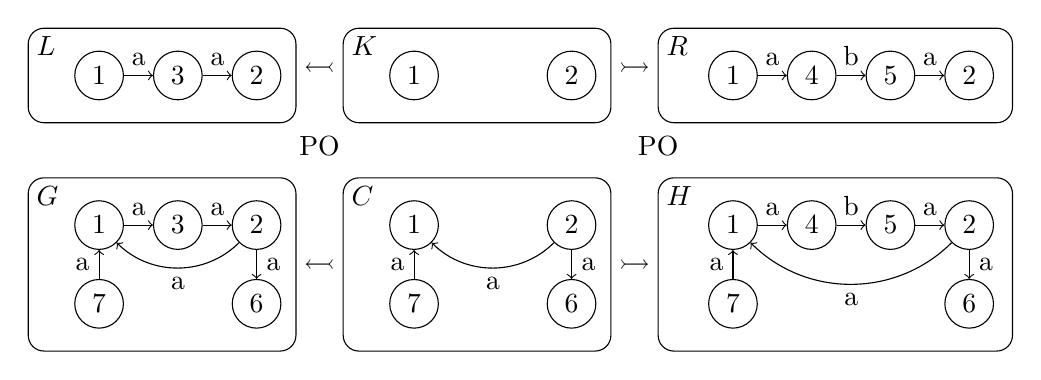
\begin{tikzpicture}
                \graphbox{\( L \)}{0mm}{-3mm}{34mm}{12mm}{2mm}{2mm}{
                    \coordinate (o) at (0mm,-8mm); 
                    \node[draw,circle] (l1) at ($(o)+(-10mm,0mm)$) {1};
                    \node[draw,circle] (l2) at ($(l1)+(2,0)$) {2};
                    \node[draw,circle] (l3) at ($(l1) + (1,0)$) {3};
                    \draw[->] (l1) -- (l3) node[midway,above] {a};
                    \draw[->] (l3) -- (l2) node[midway,above] {a};
                } 
        
                \graphbox{\( K \)}{40mm}{-3mm}{34mm}{12mm}{2mm}{2mm}{
                    \coordinate (o) at (0mm,-8mm); 
                    \node[draw,circle] (l1) at ($(o)+(-10mm,0mm)$) {1};
                    \node[draw,circle] (l2) at ($(l1)+(2,0)$) {2};
                }  
        
                \graphbox{\( R \)}{80mm}{-3mm}{45mm}{12mm}{2mm}{2mm}{
                    \coordinate (o) at (-5mm,-8mm); 
                    \node[draw,circle] (l1) at ($(o)+(-10mm,0mm)$) {1};
                    \node[draw,circle] (l2) at ($(l1)+(3,0)$) {2};
                    \node[draw,circle] (l3) at ($(l1) + (1,0)$) {4};
                    \node[draw,circle] (l4) at ($(l1) + (2,0)$) {5};
                    \draw[->] (l1) -- (l3) node[midway,above] {a};
                    \draw[->] (l3) -- (l4) node[midway,above] {b};
                    \draw[->] (l4) -- (l2) node[midway,above] {a};
                }    
        
                \graphbox{\( G \)}{0mm}{-22mm}{34mm}{22mm}{2mm}{-3mm}{
                    \coordinate (o) at (0mm,-3mm); 
                    \node[draw,circle] (l1) at ($(o)+(-10mm,0mm)$) {1};
                    \node[draw,circle] (l2) at ($(l1)+(2,0)$) {2};
                    \node[draw,circle] (l3) at ($(l1) + (1,0)$) {3};
                    \node[draw,circle] (l4) at ($(l2) + (0,-1)$) {6};
                    \draw[->] (l1) -- (l3) node[midway,above] {a};
                    \draw[->] (l3) -- (l2) node[midway,above] {a};
                    \draw[->] (l2) -- (l4) node[midway,right] {a};
                    \node[draw,circle] (l6) at ($(l1) + (0,-1)$) {7};
                    \draw[<-] (l1) -- (l6) node[midway,left] {a};
                    \draw[->] (l2) edge[out=-135,in=-45]node[midway,below] {a} (l1) ;
                }    
        
                \graphbox{\( C  \)}{40mm}{-22mm}{34mm}{22mm}{2mm}{-3mm}{
                    \coordinate (o) at (0mm,-3mm); 
                    \node[draw,circle] (l1) at ($(o)+(-10mm,0mm)$) {1};
                    \node[draw,circle] (l2) at ($(l1)+(2,0)$) {2};
                    \node[draw,circle] (l4) at ($(l2) + (0,-1)$) {6};
                    \draw[->] (l2) -- (l4) node[midway,right] {a};
                    \draw[->] (l2) edge[out=-135,in=-45]node[midway,below] {a} (l1) ;
                    \node[ draw,circle] (l6) at ($(l1) + (0,-1)$) {7};
                    \draw[<-] (l1) -- (l6) node[midway,left] {a};
                }    
        
                \graphbox{\( H \)}{80mm}{-22mm}{45mm}{22mm}{2mm}{-3mm}{
                    \coordinate (o) at (-5mm,-3mm); 
                    \node[draw,circle] (l1) at ($(o)+(-10mm,0mm)$) {1};
                    \node[draw,circle] (l2) at ($(l1)+(3,0)$) {2};
                    \node[draw,circle] (l3) at ($(l1) + (1,0)$) {4};
                    \node[draw,circle] (l4) at ($(l1) + (2,0)$) {5};
                    \node[ draw,circle] (l5) at ($(l2) + (0,-1)$) {6};
                    \node[ draw,circle] (l6) at ($(l1) + (0,-1)$) {7};
                    \draw[<-] (l1) -- (l6) node[midway,left] {a};
                    \draw[->] (l1) -- (l3) node[midway,above] {a};
                    \draw[->] (l3) -- (l4) node[midway,above] {b};
                    \draw[->] (l4) -- (l2) node[midway,above] {a};
                    \draw[->] (l2) -- (l5) node[midway,right] {a};
                    \draw[->] (l2) edge[out=-135,in=-45]node[midway,below] {a} (l1) ;
                }    
        
                \node () at (37mm,-8mm) {\( \leftarrowtail \)}; % K -> L
                \node () at (77mm,-8mm) {\( \rightarrowtail \)}; % K -> R
                \node () at (15mm,-18mm) {\(\downarrowtail \)};
                \node () at (37mm,-33mm) {\( \leftarrowtail \)};
                \node () at (37mm,-18mm) {PO};
                \node () at (58mm,-18mm) {\( \downarrowtail \)};
                \node () at (80mm,-18mm) {PO};
                \node () at (102mm,-18mm) {\( \downarrowtail \)};
                \node () at (77mm,-33mm) {\( \rightarrowtail \)}; % C -> H
            \end{tikzpicture}
            }         
        \end{center}

        An implicit occurrence of chain  \tikz[baseline=-0.5ex]{ 
        \node (x) at (0,0) {$\bullet$};  
        \node (y) at (1,0) {$\bullet$};
        \node (z) at (2,0) {$\bullet$};
        \draw[->] (x) -- node[midway,below] {a} (y) ;
        \draw[->] (y) -- node[midway,below] {a} (z) ;
    }
         \begin{center} 
        \resizebox{0.9\textwidth}{!}{
        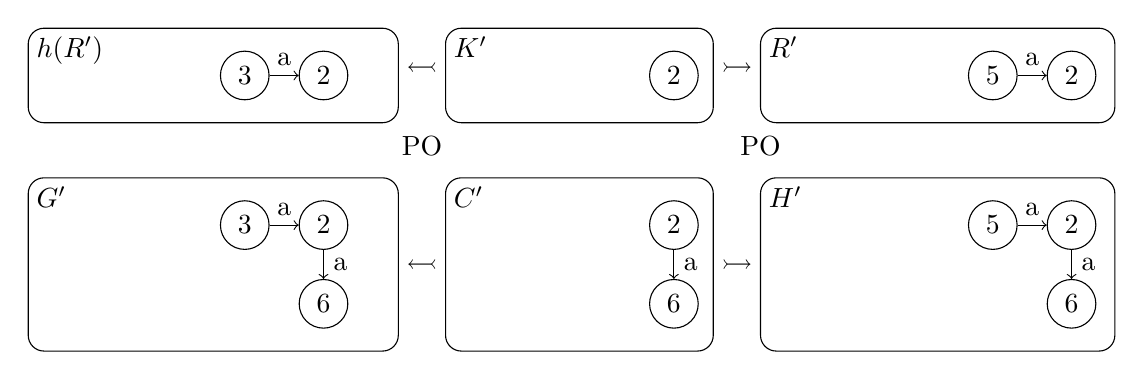
\begin{tikzpicture}
            \graphbox{\( h(R') \)}{-13mm}{-3mm}{47mm}{12mm}{2mm}{2mm}{
                \coordinate (o) at (2mm,-8mm); 
                \node[circle] (l1) at ($(o)+(-10mm,0mm)$) {};
                \node[draw,circle] (l2) at ($(l1)+(2,0)$) {2};
                \node[draw,circle] (l3) at ($(l1) + (1,0)$) {3};
                % \draw[->] (l1) -- (l3) node[midway,above] {a};
                \draw[->] (l3) -- (l2) node[midway,above] {a};
            } 
    
            \graphbox{\( R' \)}{80mm}{-3mm}{45mm}{12mm}{2mm}{2mm}{
                \coordinate (o) at (-5mm,-8mm); 
                \node[circle] (l1) at ($(o)+(-10mm,0mm)$) {};
                \node[draw,circle] (l2) at ($(l1)+(3,0)$) {2};
                % \node[draw,circle] (l3) at ($(l1) + (1,0)$) {4};
                \node[draw,circle] (l4) at ($(l1) + (2,0)$) {5};
                % \draw[->] (l1) -- (l3) node[midway,above] {a};
                % \draw[->] (l3) -- (l4) node[midway,above] {b};
                \draw[->] (l4) -- (l2) node[midway,above] {a};
            }    
    
            \graphbox{\( G'\)}{-13mm}{-22mm}{47mm}{22mm}{2mm}{-3mm}{
                \coordinate (o) at (2mm,-3mm); 
                \node[circle] (l1) at ($(o)+(-10mm,0mm)$) {};
                \node[draw,circle] (l2) at ($(l1)+(2,0)$) {2};
                \node[draw,circle] (l3) at ($(l1) + (1,0)$) {3};
                \node[draw,circle] (l4) at ($(l2) + (0,-1)$) {6};
                % \draw[->] (l1) -- (l3) node[midway,above] {a};
                \draw[->] (l3) -- (l2) node[midway,above] {a};
                \draw[->] (l2) -- (l4) node[midway,right] {a};
                % \node[draw,circle] (l6) at ($(l1) + (0,-1)$) {7};
                % \draw[<-] (l1) -- (l6) node[midway,left] {a};
                % \draw[->] (l2) edge[out=-135,in=-45]node[midway,below] {a} (l1) ;
            }    
    
            \graphbox{\( K' \)}{40mm}{-3mm}{34mm}{12mm}{2mm}{2mm}{
                \coordinate (o) at (0mm,-8mm); 
                \node[circle] (l1) at ($(o)+(-10mm,0mm)$) {};
                \node[draw,circle] (l2) at ($(l1)+(2,0)$) {2};
            } 
            \graphbox{\( C'  \)}{40mm}{-22mm}{34mm}{22mm}{2mm}{-3mm}{
                \coordinate (o) at (0mm,-3mm); 
                \node[circle] (l1) at ($(o)+(-10mm,0mm)$) {};
                \node[draw,circle] (l2) at ($(l1)+(2,0)$) {2};
                \node[draw,circle] (l4) at ($(l2) + (0,-1)$) {6};
                \draw[->] (l2) -- (l4) node[midway,right] {a};
                % \draw[->] (l2) edge[out=-135,in=-45]node[midway,below] {a} (l1) ;
                % \node[ draw,circle] (l6) at ($(l1) + (0,-1)$) {7};
                % \draw[<-] (l1) -- (l6) node[midway,left] {a};
            }  
    
            \graphbox{\( H' \)}{80mm}{-22mm}{45mm}{22mm}{2mm}{-3mm}{
                \coordinate (o) at (-5mm,-3mm); 
                \node[circle] (l1) at ($(o)+(-10mm,0mm)$) {};
                \node[draw,circle] (l2) at ($(l1)+(3,0)$) {2};
                \node[circle] (l3) at ($(l1) + (1,0)$) {};
                \node[draw,circle] (l4) at ($(l1) + (2,0)$) {5};
                \node[ draw,circle] (l5) at ($(l2) + (0,-1)$) {6};
                \node[circle] (l6) at ($(l1) + (0,-1)$) {};
                % \draw[<-] (l1) -- (l6) node[midway,left] {a};
                % \draw[->] (l1) -- (l3) node[midway,above] {a};
                % \draw[->] (l3) -- (l4) node[midway,above] {b};
                \draw[->] (l4) -- (l2) node[midway,above] {a};
                \draw[->] (l2) -- (l5) node[midway,right] {a};
                % \draw[->] (l2) edge[out=-135,in=-45]node[midway,below] {a} (l1) ;
            }    
            % \graphbox{$L$}{133mm}{-3mm}{34mm}{12mm}{2mm}{2mm}{
            %     \coordinate (o) at (0mm,-8mm); 
            %     \node[draw,circle] (l1) at ($(o)+(-10mm,0mm)$) {};
            %     \node[draw,circle] (l2) at ($(l1)+(2,0)$) {2};
            %     \node[draw,circle] (l3) at ($(l1) + (1,0)$) {5};
            %     \draw[->] (l1) -- (l3) node[midway,above] {a};
            %     \draw[->] (l3) -- (l2) node[midway,above] {a};
            % }
            % \node () at (129mm,-8mm) {\textcolor{red}{\( \rightarrowtail \)}};
            \node () at (37mm,-8mm) {\( \leftarrowtail \)}; % K -> L
            \node () at (77mm,-8mm) {\( \rightarrowtail \)}; % K -> R
            \node () at (15mm,-18mm) {\(\downarrowtail \)};
            \node () at (37mm,-33mm) {\( \leftarrowtail \)};
            \node () at (37mm,-18mm) {PO};
            \node () at (58mm,-18mm) {\( \downarrowtail \)};
            \node () at (80mm,-18mm) {PO};
            \node () at (102mm,-18mm) {\( \downarrowtail \)};
            \node () at (77mm,-33mm) {\( \rightarrowtail \)}; % C -> H
        \end{tikzpicture}
        }         
    \end{center}
\end{frame}


\begin{frame}{$X$-non-increasing rule}
    $\varphi = L \overset{l}{\leftarrowtail} K \overset{r}{\rightarrowtail} R$ : a rule

    $X \subseteq R$ : a graph

    $D(R,X)$ : subgraphs of $R$ which can form an implicit $X$-occurrence in some rewriting step

    $\varphi$ is \textcolor{red}{$X$-non-increasing rule} if 
    \begin{enumerate}
        \item For every $R_i \in D(R,X)$, there is a morphism \(h_i: R_i \rightarrowtail L \) which preserves the interface elements,
        % \item For all $R'_i \in D(R,X)$, morphism $h_i$ does not maps any non-interface element to an interface element,
        % \item Different edges $e_i \in R_i$ and $e_j \in R_j$ have different images $h_{R_iL}(e_i) \neq h_{R_jL}(e_j)$,
        % \item If $X$ has isolated nodes, then then for all $R',R'' \in D(R,X)$ and nodes $x \in R', y \in R''$, if $x \neq y$, then $h_{R'L}(x) \neq h_{R''L}(y)$.
        \item three more conditions on $h_i$
    \end{enumerate} 

    \begin{description}
        \item[Condition 1:] for every implicit $X$-occurrence in $H$, there is a corresponding implicit $X$-occurrence in $G$ with the same interface elements,
        \item[Other conditions:] different implicit $X$-occurrences in $H$ are mapped to different implicit $X$-occurrences in $G$,
    \end{description}
    for every rewriting step $G \Rightarrow H$.
\end{frame}

\begin{frame}{Main results}
    $\varphi = L \leftarrowtail K \rightarrowtail R$ : a rule

    $X \subseteq R$ : a graph
    \begin{lemma}
        For every rewriting step $G \Rightarrow H$ using $\varphi$, there are more implicit $X$-occurrences in $G$ than in $H$
        if 
        \begin{itemize}
            \item $\varphi$ is $X$-non-increasing 
        \end{itemize} 
    \end{lemma}
    \begin{theorem}[Sufficient termination condition]
        $\varphi$ terminates if
        \begin{itemize}
            \item $\varphi$ is $X$-non-increasing
            \item There are strictly more $X$-occurrences in $L$ than in $R$
        \end{itemize} 
    \end{theorem}
\end{frame}

\begin{frame}{Contribution}

    \begin{description}
        \item[Machine-checkable sufficient termination condition] 
        \item[Termination of new classes of graph rewriting systems] 
        \item[Implementation in \textbf{LyonParallel}] 
        \item[International Conference on Graph Transformation (ICGT 2025)] 
    \end{description}
\end{frame}

\subsection{Termination using Subgraph Counting with antipatterns}
\begin{frame}
   \tableofcontents[currentsubsection]
\end{frame}

\begin{frame}{Limitation of Subgraph Counting and Solution}
\begin{center} 
  \resizebox{0.7\textwidth}{!}{
  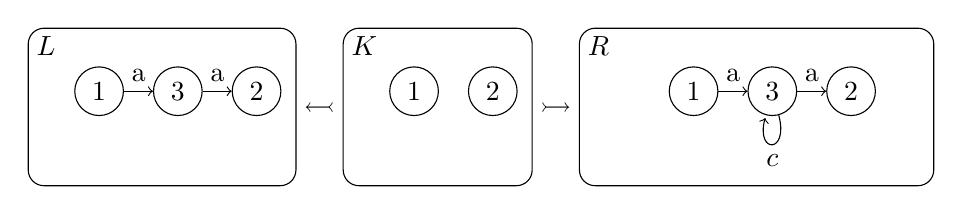
\begin{tikzpicture}
      \graphbox{$L$}{0mm}{0mm}{34mm}{20mm}{2mm}{-5mm}{
          \coordinate (o) at (0mm,-3mm); 
          \node[draw,circle] (l1) at ($(o)+(-10mm,0mm)$) {1};
          \node[draw,circle] (l2) at ($(l1)+(2,0)$) {2};
          \node[draw,circle] (l3) at ($(l1) + (1,0)$) {3};
          \draw[->] (l1) -- (l3) node[midway,above] {a};
          \draw[->] (l3) -- (l2) node[midway,above] {a};
      }     
      \graphbox{$K$}{40mm}{0mm}{24mm}{20mm}{2mm}{-5mm}{
          \coordinate (o) at (5mm,-3mm); 
          \node[draw,circle] (l1) at ($(o)+(-10mm,0mm)$) {1};
          \node[draw,circle] (l2) at ($(l1)+(1,0)$) {2};
          % \node[draw,circle] (l3) at ($(l1) + (1,0)$) {$\ $};
          % \draw[->] (l1) -- (l3) node[midway,above] {a};
          % \draw[->] (l3) -- (l2) node[midway,above] {a};
      }    
      \graphbox{$R$}{70mm}{0mm}{45mm}{20mm}{2mm}{-5mm}{
        \coordinate (o) at (0mm,-3mm); 
        \node[draw,circle] (l1) at ($(o)+(-10mm,0mm)$) {1};
        \node[draw,circle] (l2) at ($(l1)+(2,0)$) {2};
        \node[draw,circle] (l3) at ($(l1) + (1,0)$) {3};
        \draw[->] (l1) -- (l3) node[midway,above] {a};
        \draw[->] (l3) -- (l2) node[midway,above] {a};
        \draw[->] (l3) edge [loop below] node {$c$} (l3);
      }     

      \node () at (37mm,-10mm) {$\leftarrowtail$};
      \node () at (67mm,-10mm) {$\rightarrowtail$};

      % \draw[>->] (51mm,2mm) -- (52mm,3mm);
  \end{tikzpicture}
  }
\end{center}
Solution : Counting occurrences of $L$ not including in an occurrence of $R$.
\end{frame}

\begin{frame}{Contribution}
    \begin{description}
        \item[Counting subgraphs with antipatterns]
        \item[Termination of new classes of injective DPO graph rewriting systems] 
        \item[Tool available : \textbf{LyonParallel}] 
        \item[Under revision for resubmission] 
    \end{description}
\end{frame}

\section{Future Work}
\begin{frame}{Future Work}
    Graph transformation rule with negative application conditions:
    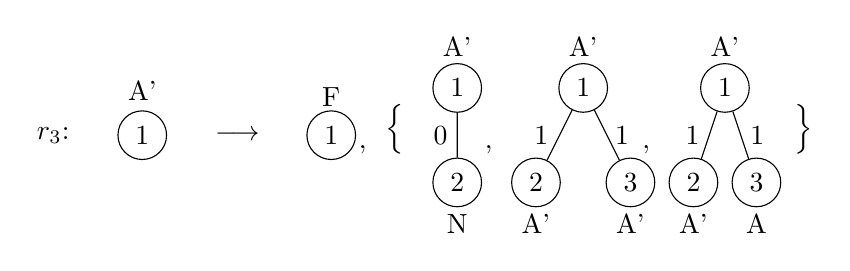
\begin{tikzpicture}[scale = 0.8]
		\draw (-1,0) node[left] {$r_3$:};
		
		\node[draw,circle] (x_1) at (0,0) {$1$} ;
		\draw (0,0.4) node[above]{A'};
		
		\draw (1,0) node[right] {$\longrightarrow$};
		
		\node[draw,circle] (x3) at (3,0) {$1$} ;
		\draw (3,0.3) node[above]{F};
		
		%context 1
		\node[draw,circle](c1_1) at (5,0.75) {$1$};
		\draw (5,1.1) node[above] {A'};
		\node[draw,circle](c1_2) at (5,-0.75){$2$};
		\draw (5,-1.1) node[below] {N};
		\draw (5,0) node[left] {$0$};
		\draw[-] (c1_1)--(c1_2);
		\draw (5.5,-0.45) node[above]{$,$};
		
		%context 2
		\node[draw,circle](c2_1) at (7,0.75) {$1$};
		\draw (7,1.1) node[above] {A'};
		\draw (6.25,-1.1) node[below] {A'};
		\draw (7.75,-1.1) node[below] {A'};
		\node[draw,circle](c2_2) at (6.25,-0.75) {$2$};
		\node[draw,circle](c2_3) at (7.75,-0.75) {$3$};
		\draw[-] (c2_1) -- (c2_2);
		\draw (6.6,0) node[left] {$1$};
		\draw (7.35,0) node[right] {$1$};
		\draw[-] (c2_1) -- (c2_3);
		\draw (8,-0.45) node[above]{$,$};
		
		%context 3
		\node[draw,circle](c3_1) at (9.25, 0.75) {$1$};
		\node[draw,circle](c3_2) at (8.75, -0.75) {$2$};
		\node[draw,circle](c3_3) at (9.75, -0.75) {$3$};
		\draw (9.25,1.1)     node[above] {A'};
		\draw (8.75,-1.1) node[below] {A'};
		\draw (9.75,-1.1) node[below] {A};
		\draw (9,0) node[left] {$1$};
		\draw (9.5,0) node[right] {$1$};
		\draw[-] (c3_1) -- (c3_2);
		\draw[-] (c3_1) -- (c3_3);
		
		
		\draw (3.5,-0.45) node[above]{$,$};
		\draw (4,-0.45) node[above]{$\Big\{$};
		\draw (10.5,-0.45) node[above]{$\Big\}$};
	\end{tikzpicture}

 Extending the technique to DPO graph rewriting systems with negative application conditions 
\end{frame} 

\end{document}